\section{Front-End Interface}
\label{sec:fei}

This section discloses an analysis and assessment of the circuitry employed in the cytometer platform. By considering the previous platforms \cite{PMID24761029, Germano2006MICROSYSTEMFB, TIM.2013.2296417}, this study introduces innovative features to enhance the MFC system performance.

\subsection{Bias Architecture}

The MR sensors, being passive elements, require biasing to ensure accurate signal measurements. The bias architecture consists of two circuit blocks: the reference voltage and the biasing topology. The reference voltage provides stability and serves as a reference for the biasing topology, which generates and supplies a known current to the sensor. By measuring the change in voltage, it is possible to determine the magnitude and direction of the magnetic field being sensed by the sensor.

The bias topology employs a combination of a Voltage-Controlled Current Source (VCCS) circuit and an emitter degenerated current mirror. The VCCS circuit converts a reference voltage into a proportional current, while the current mirror circuit replicates or mirrors this current, ensuring its independence from the sensor. The topology can be seen in Figure \ref{fig:bias-full}.

\begin{figure}[!ht]
    \centering
    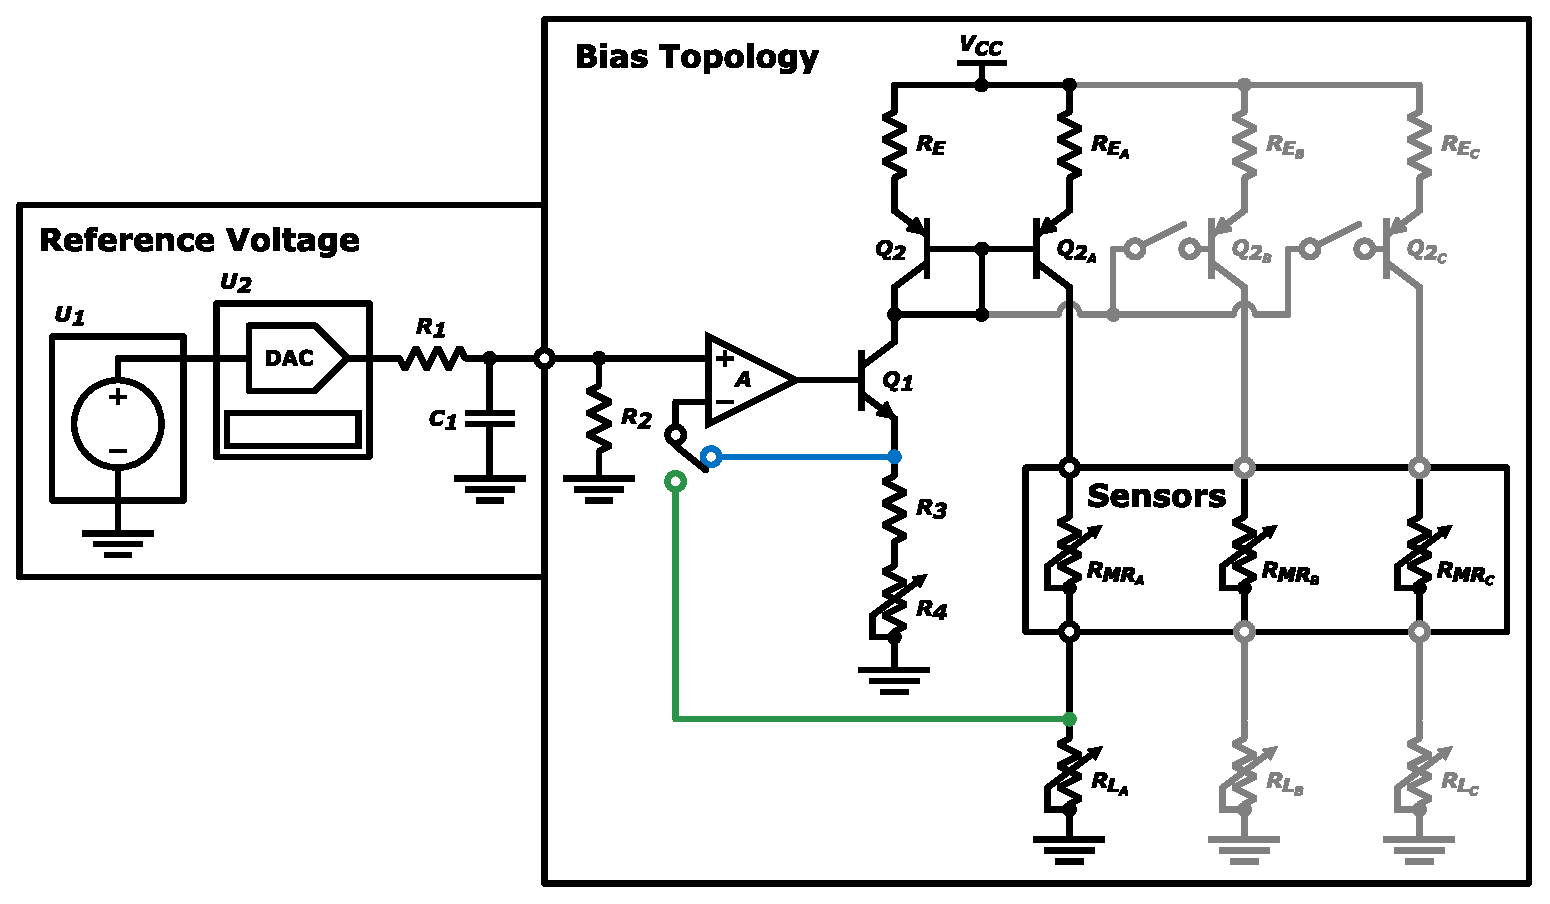
\includegraphics[width=.475\textwidth]{figs/bias_full.eps}
    \caption{Biasing architecture.}
    \label{fig:bias-full}
\end{figure}

The Figure \ref{fig:bias-full} bias circuit in the cytometer platform was designed to accommodate two different topologies: the blue line topology and the green line topology.
The blue line topology, which was used in previous versions of the cytometer, places the sensor outside the feedback loop. This topology has been proven effective and serves as the primary design choice for the bias circuit. On the other hand, the green line topology, which places the sensor inside the feedback loop, is an alternative that has not yet been validated to reduce noise. It is included in the architecture to enable further investigation and experimentation.

To achieve precise and stable biasing in electronic circuits, a voltage reference generator coupled with a digital-to-analog converter (DAC) circuit was developed (Figure \ref{fig:vref-schematic}). This approach \cite{Germano2006MICROSYSTEMFB} ensures accurate control over the output current, even in the presence of environmental factors. The DAC allows for digital adjustment of the reference voltage, providing flexibility and enabling the generation of arbitrary waveforms.

\begin{figure}[!ht]
    \centering
    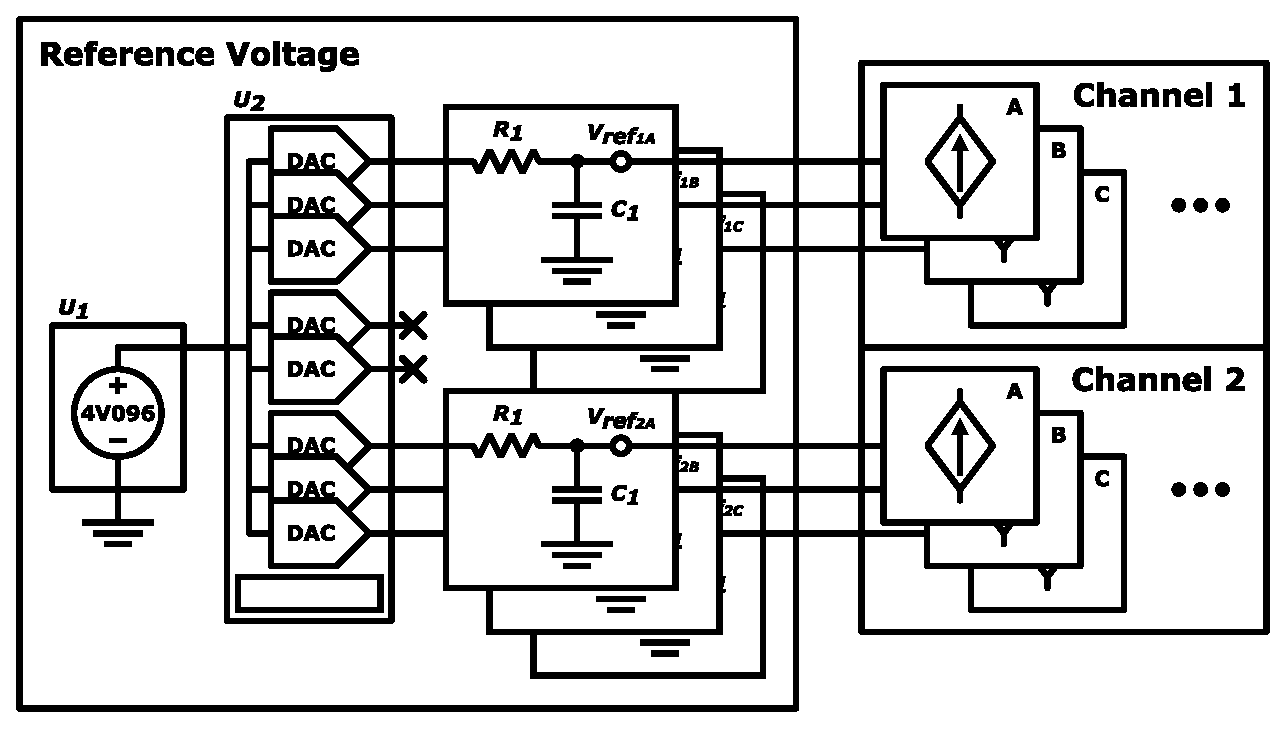
\includegraphics[width=.475\textwidth]{figs/vref.eps}
    \caption{Reference voltage schematic.}
    \label{fig:vref-schematic}
\end{figure}

The reference voltage schematic used in the interface of the cytometer platform is shown in Figure \ref{fig:vref-schematic}. Variations in the nominal resistance of the sensors may occur. To address this issue, a DAC is utilized to individually adjust the current feeding of each sensor. This allows for compensation without the need for more accurate components like precise resistors or potentiometers.

% #############################################################################
\subsection{Amplification Scheme}

In this application, magnetic particles passing through a magnetic sensor generate pulses that represent the number of analytes in the sample. The sensor signal is converted using an analog-to-digital converter (ADC) for digital processing. To ensure optimal performance and reduce quantization noise, the signal is amplified. Given that the sensor response signal is typically in the hundreds of microvolts range, the amplification scheme employed will boost the signal by a factor of 10,000.

The amplification scheme consists of two stages \cite{TIM.2013.2296417}. The first stage utilizes a differential amplifier that subtracts common voltages between input terminals, effectively reducing the impact of common noise on measurement accuracy. This stage is crucial for establishing the system's SNR. The second stage employs a non-inverting amplifier for further amplification. The circuit is completed with an anti-aliasing filter at the output. Figure \ref{fig:amp-schematic} illustrates the amplification scheme.

\begin{figure}[!ht]
    \centering
    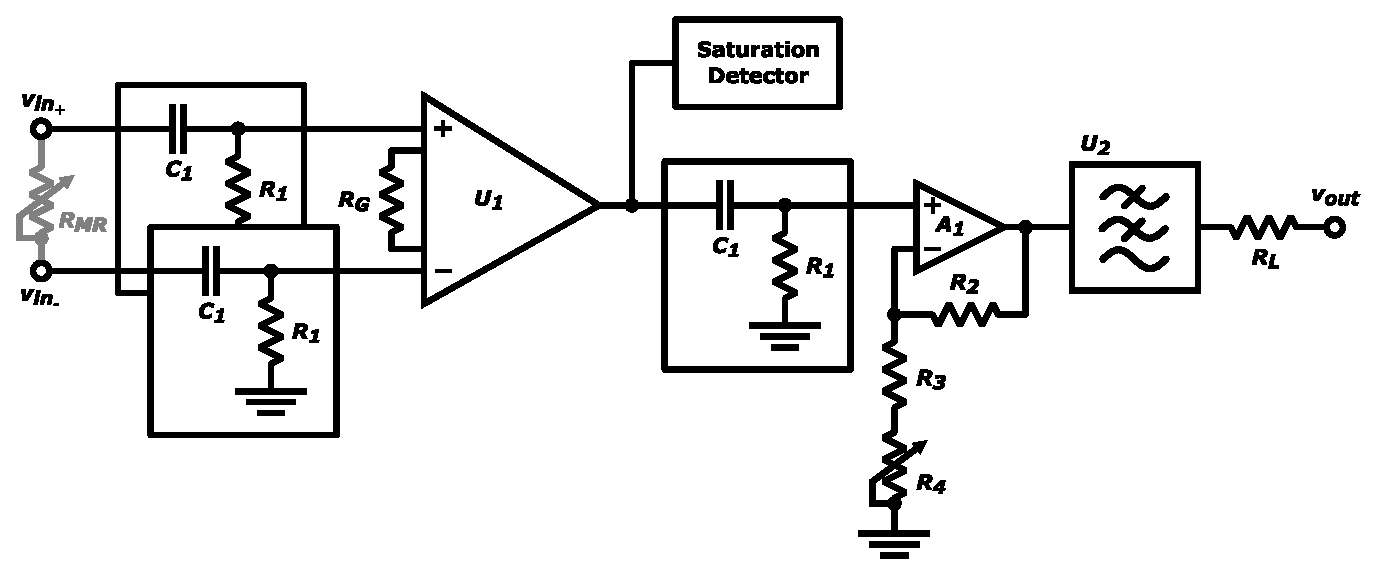
\includegraphics[width=.475\textwidth]{figs/amp.eps}
    \caption{Amplification and filtering schematic.}
    \label{fig:amp-schematic}
\end{figure}


An auxiliary circuit has been developed to address issues of signal saturation in the first stage due to noise. This circuit provides a mechanism to detect and possibly remove saturated acquired samples by alerting the user when the signal saturates. Figure \ref{fig:sat} illustrates the circuit for the "Saturation Detector" block, as shown in Figure \ref{fig:amp-schematic}. 

\begin{figure}[!ht]
    \centering
    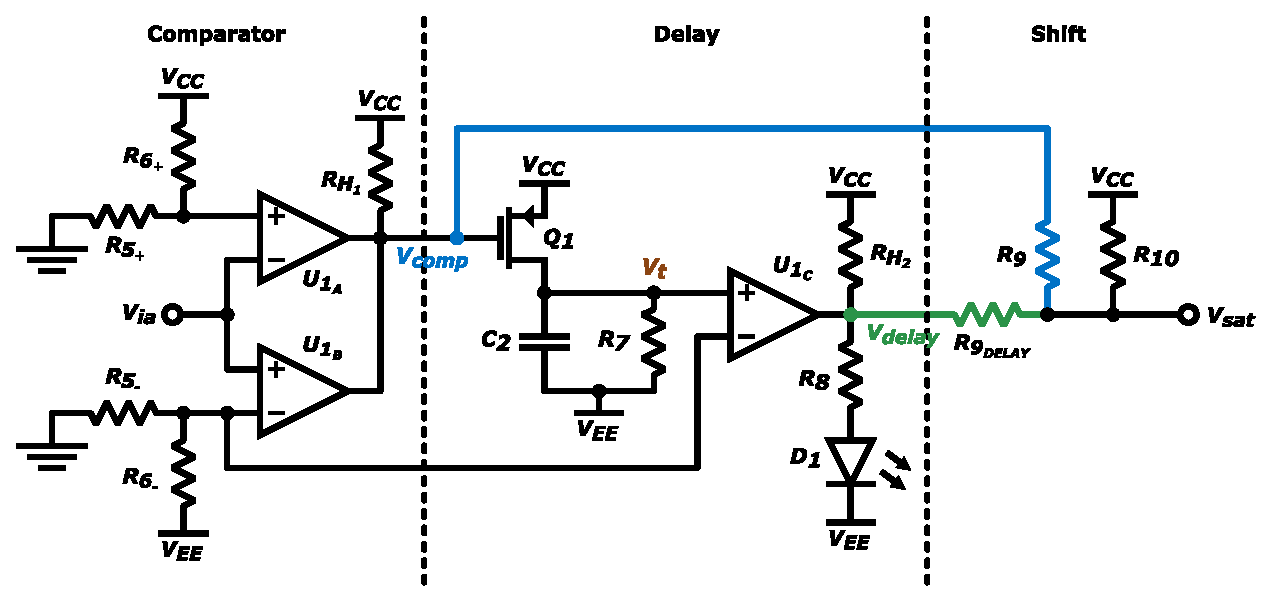
\includegraphics[width=.475\textwidth]{figs/sat.eps}
    \caption{Saturation detector circuit.}
    \label{fig:sat}
\end{figure}

The circuit in Figure \ref{fig:sat} can be divided into three segments: Comparator, Delay, and Shift. The Comparator segment is responsible for detecting when the differential amplifier saturates. The Delay segment ensures that the light-emitting diode remains on for a period of time that is noticeable to the human eye, providing a more reliable indication of saturation. Additionally, the Shift block changes the signal range. This block enables the saturated signal to be utilized in subsequent digital analysis and processing steps.
% #############################################################################

% #############################################################################
\subsection{Sensor Addressing}

The chip containing the MR sensors has been designed and manufactured at INESC, and it is connected to a custom-designed Printed Circuit Board (PCB) via wire bonding. To simplify the process of acquiring signals from the sensors, a sensor addressing module has been implemented. This module utilizes multiplexers to enable seamless switching between sensors and improve the functionality of the cytometer platform.

The implemented multiplexers enable the selection of 4 out of the 28 sensors on the chip. With 6 analog channels on the board, incorporating biasing and amplification, a total of 26 sensors can be utilized by the system. Figure \ref{fig:sensormux} shows the multiplexing circuit applied to one analog channel.

\begin{figure}[!ht]
    \centering
    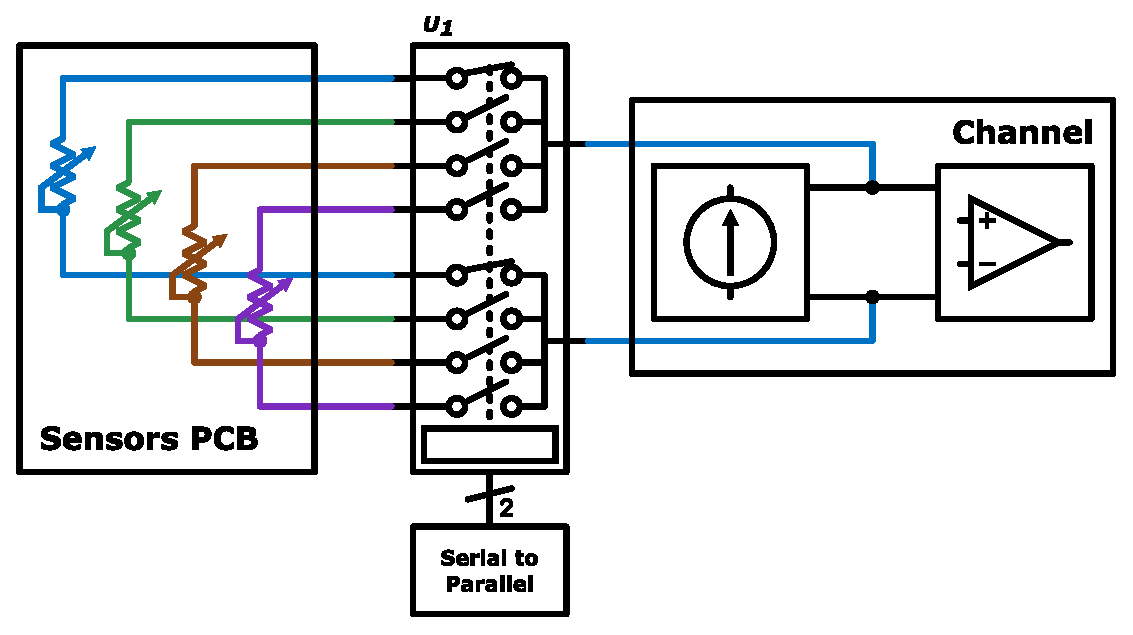
\includegraphics[width=.475\textwidth]{figs/sensormux.eps}
    \caption{Sensor addressing module.}
    \label{fig:sensormux}
\end{figure}

Figure \ref{fig:sensormux} provides a schematic diagram of the circuit used in the module and illustrates its integration into the cytometer system. The diagram shows that the first inputs of either output are selected, as indicated by the closed switch. This configuration routes the signal from the blue sensor to the output of the multiplexer, which then connects to the output of the biasing topology and the input of the amplification scheme.

To minimize the number of inputs required for the multiplexers that are using parallel communication, a circuit utilizing shift registers was developed. The Figure \ref{fig:s2p} circuit converts the parallel communication into a Serial Peripheral Interface (SPI), which reduces the number of required inputs.

\begin{figure}[!ht]
    \centering
    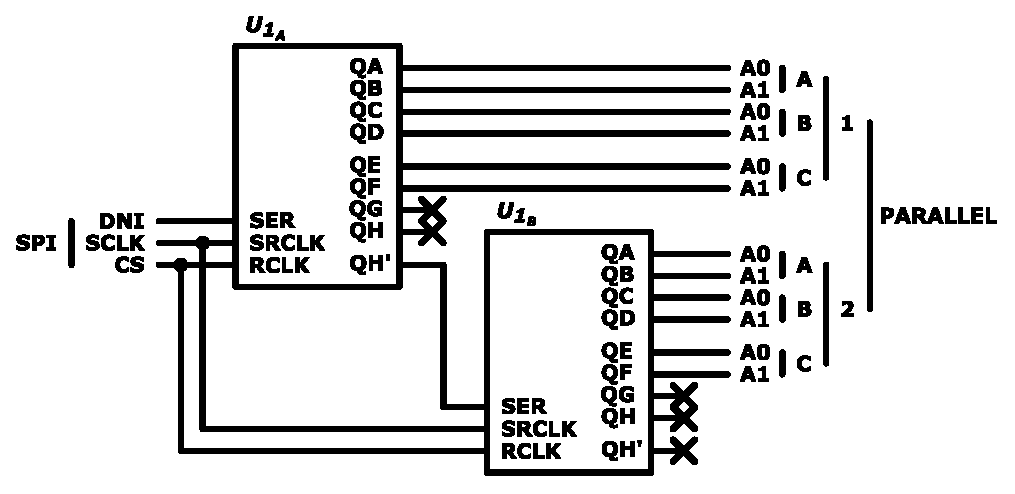
\includegraphics[width=.475\textwidth]{figs/s2p.eps}
    \caption{Serial to parallel converter circuit.}
    \label{fig:s2p}
\end{figure}

In future versions of the cytometer platform, it is recommended to use different multiplexers controlled via SPI. If such multiplexers are used, the current module converting serial communication to parallel form may become obsolete and should be removed.
% #############################################################################

% #############################################################################
\subsection{Communication Translator}

The cytometer platform includes level shifters to ensure compatibility with different controlling or data acquisition systems. These level shifters separate and convert the voltage signals to match the operating voltage of the respective devices, facilitating seamless communication and data exchange between the platform and external systems. Additionally, the platform is equipped with multiple inputs and outputs to enable efficient operation and information gathering from the board. All the signals can be found in Figure \ref{fig:level-shifters}.

The cytometer PCB was designed to connect to a Field-Programmable Gate Array (FPGA) that performs real-time Digital Signal Processing (DSP). This integration with the FPGA is expected to enhance the system's SNR and resolution. The FPGA carries out initial event detection and stores the events as a bitstream for subsequent preprocessing.

\begin{figure}[!ht]
    \centering
    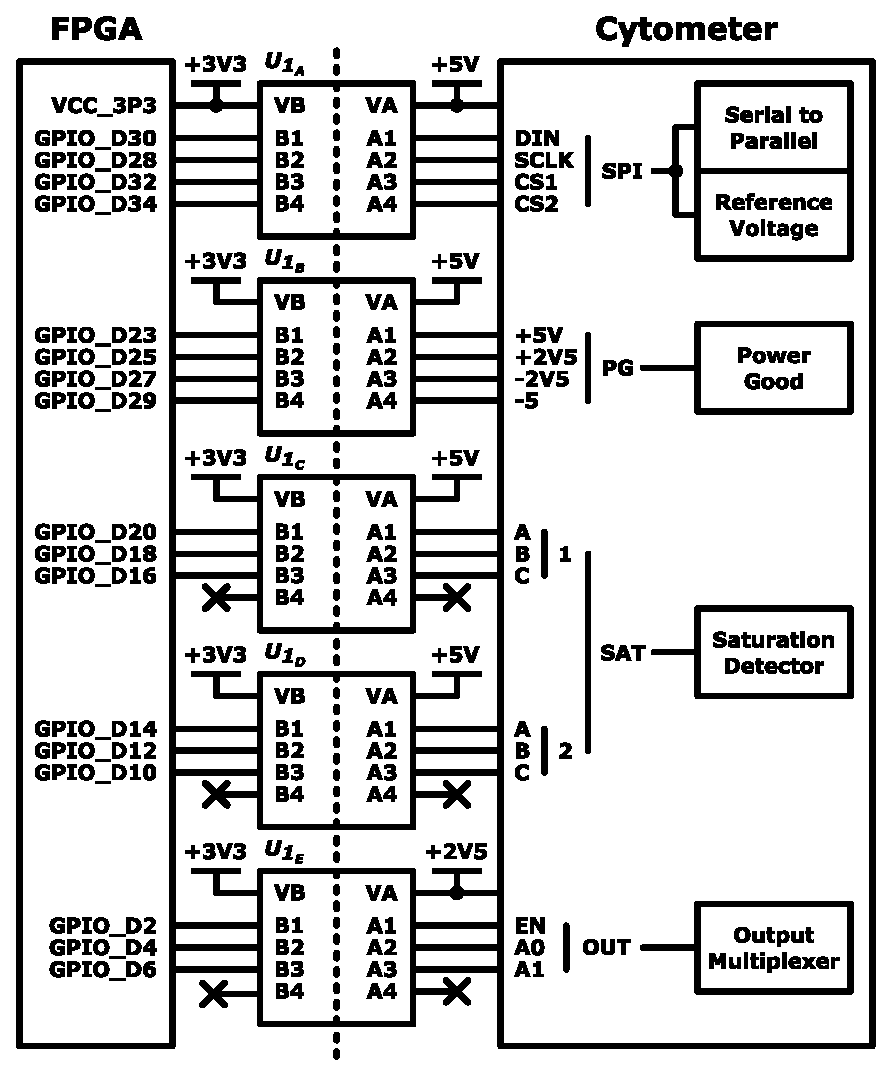
\includegraphics[width=.475\textwidth]{figs/comms.eps}
    \caption{Level shifters circuit.}
    \label{fig:level-shifters}
\end{figure}

Figure \ref{fig:level-shifters} depicts all the blocks that provide or need signals. The SPI communication protocol will be used by two circuit blocks: the serial-to-parallel block and the reference voltage block. Each block has its own chip-select signal. The serial-to-parallel block converts the serial protocol into bits that can be understood by the multiplexers in the sensor addressing circuit. The power good block, although not introduced yet, assesses whether the supply rails have sufficient voltage for the proper operation of the circuits. The FPGA can use this information to determine if the cytometer is ready to receive instructions. The saturation detector block provides information to the real-time DSP by identifying saturated signals during the amplification scheme, ensuring that such samples are not used in subsequent processing steps.
% #############################################################################

% #############################################################################
\subsection{Output Multiplexing}

To overcome the limitation of having only 2 ADCs available on the THDB-ADA acquisition board, a dedicated circuit was developed (Figure \ref{fig:outmux}) to multiplex the 6 analog channels of the cytometer platform into 2 outputs. This multiplexing circuit efficiently addresses the challenge by allowing the sharing of ADCs across multiple channels, effectively maximizing the utilization of the available resources. By multiplexing the channels, the cytometer platform can still acquire data from all 6 channels, ensuring comprehensive data collection and analysis.

\begin{figure}[!ht]
    \centering
    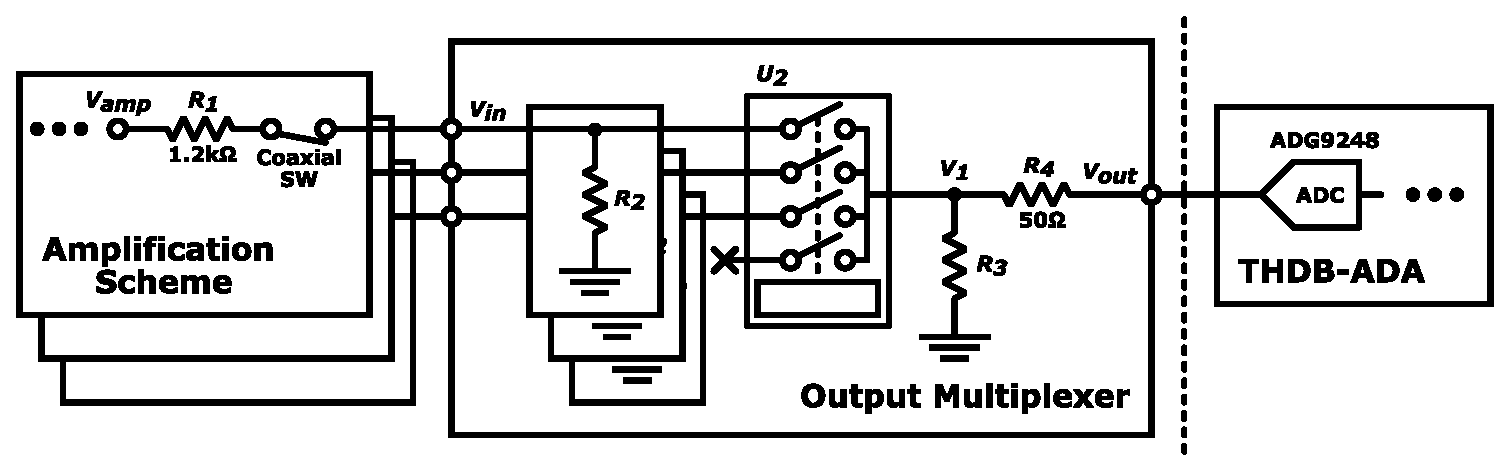
\includegraphics[width=.475\textwidth]{figs/outmux.eps}
    \caption{Output multiplexer circuit.}
    \label{fig:outmux}
\end{figure}

The circuit depicted in Figure \ref{fig:outmux} demonstrates the implementation of output multiplexing in the developed cytometer platform. Although the picture shows a single channel, it should be understood that this circuit is replicated twice to accommodate the two channels in total. To ensure maximum sampling rate of the ADCs, multiplexers with switching times lower than the sampling period were carefully selected for the purpose of channel multiplexing. If any of the inputs exceed the maximum or minimum supply voltage, the multiplexer clamps, effectively shutting down. In such cases, crosstalk may occur between the selected channel and the input signal that exceeded the supply voltage. Therefore, it is crucial for the circuit to ensure that the input signals stay within the range of $\mathrm{\pm2.5~V}$, and the output does not exceed the $\mathrm{\pm1~V}$. This limitation is necessary because the acquisition board ADCs cannot handle higher voltages, as previously specified. The voltage reduction is achieved through a two-step process using voltage dividers. This design approach ensures compatibility with the previous version of the cytometer, utilizing the same ADC and enabling broader compatibility beyond FPGA usage.

This module is designed to function independently, with inputs being connected through
SMA connectors. The amplification scheme can be detached from this circuit using the coaxial switches mentioned in the relevant section. This unique feature allows this module to be utilized as a mini-board for other applications.
% #############################################################################

% #############################################################################
\subsection{Power Supply}

Power supply is a critical aspect of electronic circuits as it enables the proper functioning of circuit components and the generation of desired electrical signals. This section explores the power circuits in detail to ensure optimal performance, reliability, and longevity of the electronic system.

The cytometer platform requires four supply rails: $\mathrm{+5~V}$, $\mathrm{+2.5~V}$, $\mathrm{-2.5~V}$, and $\mathrm{-5~V}$. To enhance flexibility, the circuit is designed to accommodate multiple power sources. Batteries offer reliability, minimal noise, and portability, making them ideal for experiments and field use. A laboratory power supply can be used as an alternative, although it may introduce higher levels of noise and reduce portability. The FPGA can also provide power, simplifying the setup process and reducing complexity. Universal Serial Bus (USB) power can also be utilized, using power banks or direct connections to a computer. Figure \ref{fig:pwr-sources} illustrates the transformation of power sources into the necessary power rails for the PCB.

\begin{figure}[!ht]
    \centering
    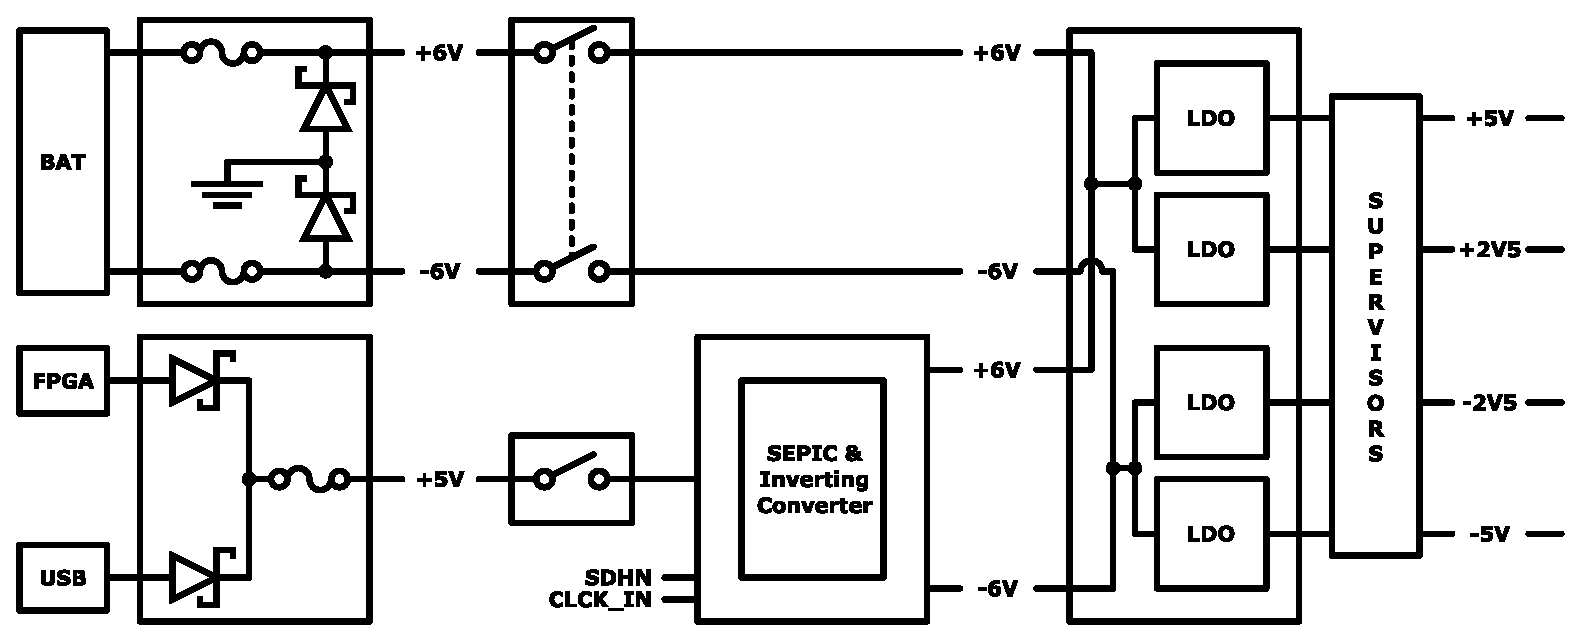
\includegraphics[width=.475\textwidth]{figs/power.eps}
    \caption{Power circuit diagram.}
    \label{fig:pwr-sources}
\end{figure}

As depicted in Figure \ref{fig:pwr-sources} the different power sources have different paths. Measures are implemented to ensure safe and efficient utilization of these power sources. A power protection circuit safeguards subsequent circuits when the battery is wrongly connected. The diodes isolates the FPGA and USB power sources to prevent current flow between them. A DC/DC converter, specifically a SEPIC and inverting circuit, boosts the signal and inverts the polarity of the rail generating $\mathrm{\pm6~V}$ rails. A Low-dropout (LDO) regulator circuit adjusts these input voltages to meet PCB requirements, providing a stable and reliable power supply. The power supervisor circuit, after the LDOs, in the cytometer platform PCB adds an extra layer of protection and user awareness, ensuring that power supply conditions are monitored and potential issues are detected in a timely manner.

By understanding and implementing these power conversion and protection mechanisms, the PCB can efficiently utilize available power sources and provide regulated voltages for proper circuit functionality. This ensures the reliable operation of the cytometer platform in various operating scenarios.
% #############################################################################

